\documentclass[a4paper]{report}
\usepackage[a4paper, left=1.3in, right=1.3in, top=1in, bottom=1in]{geometry}
\usepackage{tabularx}
\usepackage{amsmath}
\usepackage{graphicx}
\usepackage{subcaption}
\usepackage{cite}
\usepackage{svg}
\usepackage[utf8]{inputenc}
\usepackage[T1]{fontenc}
\usepackage{float}
\usepackage{multirow}
\usepackage{listings}
\usepackage{array}
\newcolumntype{P}[1]{>{\centering\arraybackslash}p{#1}}

\usepackage{indentfirst}
\usepackage{tensor}
\usepackage{amssymb}
\allowdisplaybreaks
\usepackage{bm}
\newcommand{\at}[2][]{#1|_{#2}}
\newcommand\numberthis{\addtocounter{equation}{1}\tag{\theequation}}
\newcommand\norm[1]{\left\lVert#1\right\rVert}
\usepackage{caption}
\captionsetup[lstlisting]{font={small}}
\captionsetup[figure]{font=small, labelfont={it}, textfont={it}}
\captionsetup[table]{font=small, labelfont={it}, textfont={it}}
\usepackage{breqn}
\usepackage{verbatim}
\usepackage{wasysym}
\usepackage{wrapfig}
%%%%%%%%%%%%%%%%%%%%%%%%%%%%%%%%%%%%%%%%%%%%%%%%%%%%%%%%%%%%%%%%%%%%%%%%%%%%%%%%%%%%%%%%%%%%%%
% DA QUI IN GUI RIGUARDA IL COLORE DEL CODICE CHE RIPORTIAMO, SE NON INTERESSA SI CANCELLA
%%%%%%%%%%%%%%%%%%%%%%%%%%%%%%%%%%%%%%%%%%%%%%%%%%%%%%%%%%%%%%%%%%%%%%%%%%%%%%%%%%%%%%%%%%%%%%
\usepackage{listings}
\usepackage{color}
\definecolor{lightgray}{rgb}{0.98,0.98,0.98}
\definecolor{darkgray}{rgb}{.4,.4,.4}
\definecolor{orange}{rgb}{0.9, 0.1, 0}
\definecolor{green}{rgb}{0.2, 0.8, 0}



\lstdefinelanguage{JavaScript}{
  keywords={typeof, new, true, false, catch, function, return, null, catch, switch, var, if, in, while, do, else, case, break, for, let},
  keywordstyle=\color{blue}\bfseries,
  ndkeywords={class, export, boolean, throw, implements, import, this},
  ndkeywordstyle=\color{darkgray}\bfseries,
  identifierstyle=\color{black},
  sensitive=false,
  comment=[l]{//},
  morecomment=[s]{/*}{*/},
  commentstyle=\color{green}\ttfamily,
  stringstyle=\color{orange}\ttfamily,
  morestring=[b]',
  morestring=[b]"
}

\lstset{
   language=JavaScript,
   backgroundcolor=\color{lightgray},
   extendedchars=true,
   basicstyle=\footnotesize\ttfamily,
   showstringspaces=false,
   showspaces=false,
   numbers=left,
   numberstyle=\footnotesize,
   numbersep=9pt,
   tabsize=2,
   breaklines=true,
   showtabs=false,
   captionpos=b
}             
%%%%%%%%%%%%%%%%%%%%%%%%%%%%%%%%%%%%%%%%%%%%%%%%%%%%%%%%%%%%%%%%%%%%%%%%%%%%%%%%%%%%%%%%%%%%%%
%%%%%%%%%%%%%%%%%%%%%%%%%%%%%%%%%%%%%%%%%%%%%%%%%%%%%%%%%%%%%%%%%%%%%%%%%%%%%%%%%%%%%%%%%%%%%%

\usepackage{makecell}
\usepackage{hyperref}  % importare per ultimo https://www.overleaf.com/learn/latex/Hyperlinks
\definecolor{dkgrey}{rgb}{0.2, 0.2, 0.2}
\hypersetup{
    colorlinks=true,
    linkcolor=dkgrey,
    urlcolor=cyan,
		pdftitle={IG Report: "Masks of Babylon"},
}
\graphicspath{ {./images} }
% collegamento ipertestuale che scrive anche nome e numero del capitolo/sezione.
% Source: https://tex.stackexchange.com/questions/121865/nameref-how-to-display-section-name-and-its-number
\newcommand*{\fullref}[1]{\hyperref[{#1}]{\autoref*{#1}: \nameref*{#1}}}

\setlength{\parindent}{0pt}

\begin{document}

%\title{Masks of Babylon}
\makeatletter
%\let\thetitle\@title
\let\theauthor\@author
\let\thedate\@date
\makeatother

\begin{titlepage}
	\centering
    \vspace*{0.5 cm}
    \includegraphics{images/sapienza-MLred-pos}\\[1.0 cm]	% University Logo
    \vspace*{-0.5cm}
    \textsc{\large Facoltà di \\Ingegneria dell'Informazione, Informatica e Statistica}\\[0.5 cm]	% Department Name
    \textsc{\large Dipartimento \\di Ingegneria Informatica, Automatica e Gestionale}\\[0.5 cm]	% Department Name
    \textbf{\large Interactive Graphics}\\[0.1 cm]
    \textbf{\large Final project}\\[2.0 cm]
    \textsc{\large A.Y. 2020/21}\\[2.0 cm]
    { \fontsize{20.74pt}{18.5pt}\selectfont\bfseries \par } % \thetitle
    % \vspace*{5.6cm}
    \begin{figure}[htbp]
    \centering
    \includesvg{images/Masks_of_Babylon_1_purple.svg}
    \end{figure}
    \vspace*{3cm}
	\begin{minipage}{0.4\textwidth}
		\begin{flushleft} \large
			\emph{Professor:}\\
			Marco Schaerf\\
		\end{flushleft}
	\end{minipage}~
	\begin{minipage}{0.4\textwidth}
		\begin{flushright} \large
			\emph{Students (alphabetical order):} \\
            Giovanni Pecorelli 1799865\\
            Francesco Petri 1797147\\
            Jacopo Rossi 1801667\\
            Giacomo Venneri 1810169
		\end{flushright}
	\end{minipage}\\[2 cm]
\end{titlepage}

\tableofcontents
\newpage

\setlength{\parskip}{1em}

%!TEX root = main.tex

\chapter{Introduction}

\textbf{\textit{Masks of Babylon}} is a project inspired by classic turn-based role-playing videogames (RPG) which lets the user play a simplified game of this genre. The player can explore a labyrinth, find items, and fight enemies.

\section{Libraries used}

The project is built entirely with \textbf{BabylonJS}, an open-source library and rendering engine running on top of WebGL. It offers a variety of features, including:

\begin{itemize}
    \item Rendering a scene with a variety of materials
    \item Support for different kinds of textures, including color, normal, specular, metallic-roughness, and emission
    \item Organizing a scene hierarchically
    \item Loading external models in the glTF format and the associated textures
    \item Animation of simple and complex objects, with support for keyframes and easing functions, as well as bones for complex objects
    \item User interaction through keyboard/mouse controls, mesh picking, and GUI (through the additional Babylon GUI module)
    \item Lighting and shadows
    \item Mesh instancing and cloning
\end{itemize}

We also use \texttt{pep.js} to get a uniform framework for pointer events across all platforms.

No other external libraries were used: in particular, our project has no need for a physics engine since it does not aim to simulate it, nor does it need extra animation libraries such as \texttt{tween.js} since Babylon covers that range of features on its own.

\section{Other tools used}

\begin{itemize}
    \item \textbf{Blender:} 3D model editor which we used to make a few simple new models, adapt some of the models found online to the needs of our project, and prototype the animation keyframes for the complex models before writing them out in the code.
    \item \textbf{GIMP/Photoshop:} advanced image editors which we used to prepare some textures found online for use in our project and to combine some of those textures into new ones to reduce the number of materials of certain objects.
    \item \textbf{Inkscape:} SVG editor used to adapt some SVG icons found online to our project, including coloring them, and to create single SVG files holding multiple such icons.
    \item \textbf{Babylon Sandbox:} tool developed by the BabylonJS community which we used to preview how Babylon would process the objects contained in some glTF files.
    \item \textbf{Overleaf:} online LaTeX editor, used to make this document.
\end{itemize}

\section{Browser compatibilty}

The project has been tested on the following browsers:

\begin{itemize}
    \item Google Chrome
    \item Mozilla Firefox
    \item Opera
    \item Microsoft Edge
\end{itemize}

No particular problem has been encountered while testing the game on any of these platforms.

%!TEX root = main.tex

% https://tex.stackexchange.com/questions/24066/start-new-chapter-on-same-page/24068#24068
{
\let\clearpage\relax

\chapter{User Manual}
}

This section describes how the user can interact with our application.

The core of the game alternates between two phases: in the \textit{exploration phase}, the user can explore the play environment, called the "dungeon"; while the \textit{battle phase} is about fighting an enemy in a turn-based battle by selecting the actions to perform each turn. Furthermore, this application starts with a main menu that displays a summary of the controls and offers a few options for the user to set, and there is a simple ending scene shown when the player reaches their objective at the end of the dungeon.

\section{Premise of the game}

The user plays the role of a young adventurer who must recover an artifact from the lair of an evil monster.

The goal of the game is therefore to explore this dungeon, clear the way of any obstacles such as enemies and locked doors, and ultimately reach the final room and defeat the "boss" monster.

\section{Main Menu}

The main menu is a simple screen realized entirely with the Babylon.js UI module. The user can start the game by clicking the large button at the center of the screen, and they can review the controls at the left-hand side of the screen. \textit{However, the menu screen is not very responsive, so if it does not fit the screen we advise using the zoom out feature of the browser.}

The right-side panel shows the options that can be set:

\begin{itemize}
    \item \textbf{Difficulty.} Changes the difficulty level of the battles. \textit{Normal} is the default difficulty, while in \textit{Hard} mode the enemies will have more HP and higher attack power.
    \item \textbf{Sensibility.} Sets the mouse sensibility on all axes and in all scenes, dungeon and battle alike. Three levels are available.
    \item \textbf{Shadows.} Allows the user to turn the shadows on or off in all scenes, and to choose their quality level if on. \textit{Off} disables shadows entirely. \textit{Low Quality} turns on the shadows, but using a low-resolution shadow map and no smoothing filters. As a result, the shadows will appear blocky, but they won't have much of an impact on performance if the user has a lower-end graphics card. \textit{High quality} turns on the shadows with a higher resolution and smoothing filters for a more pleasant look which may require more powerful hardware.
\end{itemize}

\begin{figure}[H]
    \centering
    \includegraphics[width=0.9\textwidth]{images/ch2/main-menu.png}
    \caption{Main menu screen}
    \label{fig:main-menu}
\end{figure}

\section{Exploration Phase}

\subsection{Introduction and controls}
\label{sub:exploration-controls}

In this mode the dungeon is shown in a first-person view. The user can move and look around in multiple ways:

\begin{itemize}
    \item \textbf{WASD keys:} Move forward, left, backward and/or right with respect to where the camera is looking.
    \item \textbf{Arrow keys:} \textit{Up} and \textit{Down} move forward or backward, while \textit{Left} and \textit{Right} allow the user to turn around in their respective direction.
    \item \textbf{Mouse:} \textit{Hold the left button and move the mouse} to look around.
    \item \textbf{Shift:} Hold this key while moving with WASD or Arrows to walk faster.
\end{itemize}

Therefore the player can choose their preferred control scheme: moving with WASD and turning with the mouse, or using the arrows to do both at once but sacrificing some freedom.

\subsection{Interacting with objects}

Several interactable objects can be found throughout the play environment. Each of them can be interacted with by getting close to it and clicking on it with the left mouse button.



The following is a list of all interactable objects found in the project:

\begin{itemize}
    \item \textbf{Keys.} Click on a key to pick it up and carry it. The key can be used later to open a lock of the same color.
    \item \textbf{Locks.} These devices are always mounted on gates that block the way forward. If the user clicks on a lock while holding a key of the same color, the lock opens and the obstacle is removed. Otherwise, nothing happens.
    \item \textbf{Doors.} These objects can be used to move between the several areas the dungeon is composed of. Click on a door to go to the area it connects to.
    \item \textbf{Enemies.} Click on an enemy to enter the \textit{Battle Phase} and fight it. Enemies block the way until they are defeated.
\end{itemize}

These interactive objects can also be identified because the cursor changes from the default arrow to a pointing hand when hovering on one of them while the player is close enough to interact with it. \textit{However, because the \texttt{BABYLON.ActionManager} object, which we used to implement this behavior, offers events for the pointer entering or exiting a mesh but not for the pointer moving inside a mesh without entering or leaving, the cursor will not change if the user approaches the object from afar while keeping the cursor on it. The cursor will change as normal if the user then moves the cursor away from the interactive object and then back on it.}

\subsection{The story screen}

The very first time the user enters the dungeon after starting the game, a simple screen explaining the premise described above will be shown. The user only needs to read it and click OK to start playing.

\section{Battle Phase}

In this mode the player can fight one enemy in a turn-based battle, i.e. the two characters alternate taking actions to attack one another or to mitigate enemy attacks. The enemy won't attack during the player's turn no matter how much time the user takes to think, and neither character can act more than once before the other gets to take their turn.

The scene is shown in a side-view with the player character on the left and the enemy on the right, but the user can orbit the camera freely to explore a variety of third-person perspectives. UI elements in the corners of the screen show the amount of Health Points (HP) of each character.

The goal of a battle is to defeat the enemy character by reducing its HP to zero with attacks while avoiding that the player character's own HP fall to zero under the enemy's strikes.

\subsection{Battle actions}

During their turn, the user can select one action to take by clicking one of the four buttons that appear in the lower left area of the screen. If the user hovers on one of the buttons without clicking, they can read a short description of that action in the text box below.

Each action causes one or more animations and/or light effects to play and has some effect on the state of the battle.

The actions available to the player are the following:

\begin{itemize}
    \item \textbf{Attack.} The player character performs a simple slashing animation with his sword and causes the enemy to recoil because of the hit. The enemy takes a little damage to their HP.
    \item \textbf{Charge.} The player character transitions to a defensive pose, and then transitions back to their idle pose at the start of the next turn. This action causes the player to turn on their \textit{charge state}, which is needed to perform other actions, and halve any damage taken during that turn.
    \item \textbf{Fireball.} The player character performs a more elaborate animation in which he throws a fireball at the enemy, causing them to recoil and take higher damage to their HP. The player needs to have their \textit{charge state} on to perform this action, and executing it will turn it off again.
    \item \textbf{Prayer.} The player character performs an animation that represents him casting a healing spell and  recovers some HP, but he needs to have his \textit{charge state} on to perform this action, and executing it will turn it off again.
\end{itemize}

\subsection{The enemy turn}

Each enemy has two actions available to them: a normal attack and a stronger special attack. The enemy chooses an action at random on each of their turns, but the probability of choosing one or the other is influenced by the last action taken by the user: if the player used \textit{Fireball}, a strong attack, the enemy is more likely to retaliate with their own special attack; conversely, if the player used a non-offensive action like \textit{Charge} or \textit{Prayer}, the enemy will be more likely to use the normal attack.\\
Thus the user can also consider the most likely enemy response when planning their next move.

\subsection{Camera control}

At any time during the battle, the user can hold the left mouse button over the battle scene and move the cursor to orbit the camera around the arena.

A button on the bottom right corner of the screen allows the user to lock or unlock the camera: while it is locked, it returns to the default side view and cannot be moved this way until it is unlocked again.

\subsection{The victory screen}

This is a simple UI that appears when the player defeats the enemy by reducing its HP to zero.

Its purpose is to inform the player of the victory, and it includes a button that the user can click to proceed in the game.

\subsection{The game over screen}

This is a simple UI that appears when the player is defeated by the enemy to inform the user of the unfortunate event.

The user can click one of three buttons to decide what to do next:

\begin{itemize}
    \item \textbf{Retry the fight.} Restarts the current battle from the beginning.
    \item \textbf{Skip this battle.} Allows the player to skip the current battle as though they had won, in order to let any user see all the content in the project regardless of their expertise in turn-based RPG battles.
    \item \textbf{Quit to main menu.} Lets the user return to the main menu. All progress made through the dungeon will be lost.
\end{itemize}

\section{Ending scene}

Once the user defeats the boss of the dungeon, a simple scene is displayed to show the player character finally recovering the artifact he is looking for, and to inform the user they have completed the game.

The only interaction possible in this scene is a limited orbiting of the camera which works like in the battle scene, and a button in the lower right corner that lets the user return to the main menu.

%!TEX root = main.tex

% https://tex.stackexchange.com/questions/24066/start-new-chapter-on-same-page/24068#24068
{
\let\clearpage\relax

\chapter{Models}
}

\section{Hierarchical models}

The player and enemy characters are represented by complex models that include a hierarchy of bones to drive the animation of different parts of the mesh.

\subsection{Makoto, the player character}

The model for the player character is named \textit{Makoto} and has the form of a stylized human holding a sword. The model and its bones are shown in \autoref*{fig:makoto-bones}.\footnote{The bones have been enlarged in order to make it possible to see them in the first place. In the real model, all bones are point-like and pointing up.}

\begin{figure}[H]
    \centering
    \includesvg[width=\textwidth]{images/ch3/Grafo-Makoto.svg}
    \caption{Hierarchy tree of Makoto's bones}
    \label{fig:makoto-graph}
\end{figure}

\begin{wrapfigure}[23]{r}{0.4\textwidth}
    \centering
    \includegraphics[width=0.4\textwidth]{images/ch3/Makoto-Bones-v2.png}
    \caption{Makoto's model with his bones shown. The bones have been colored by group (root and spine, legs, arms, head)}
    \label{fig:makoto-bones}
\end{wrapfigure}

Makoto's model is made of one mesh which is fully UV-mapped to one color texture. We also generated a roughness map from that texture in order to make the sword in his hand and the earphones around his shoulder shinier and more metallic-looking, although this effect is hard to see.

Because half of Makoto's face is covered by his hair, we used this model flipped along the X axis in order to make his better profile visible in the default view of the battle scene, where the player is placed on the left side of the screen and facing right.

The animation of the mesh is driven by the hierarchy of bones described in \autoref*{fig:makoto-graph}. They are directly mapped to TransformNode and Bone objects in the Babylon environment. Specifically, this is a list of the relevant bones for animating:

\begin{itemize}
    \item \textbf{rot} and \textbf{Bip01} are the top nodes. The former is located at the base of the model, the latter approximately at his waist.
    \item \textbf{Bip01_Spine} and \textbf{Bip01_Spine1} control the torso and chest.
    \item \textbf{Bip01_L_Thigh}, \textbf{Bip01_L_Calf} and \\ \textbf{Bip01_L_Foot} control the respective parts of the left leg. Similarly for the right counterparts.
\end{itemize}

\begin{itemize}
    \item \textbf{Bip01_L_Clavicle}, \textbf{Bip01_L_UpperArm}, \textbf{Bip01_L_Forearm} and \\ \textbf{Bip01_L_Hand} control the corresponding parts of the left arm. Similarly for the right counterparts.
    \item \textbf{weapon} controls the sword.
    \item \textbf{Bip01_Neck} and \textbf{Bip01_Head} control the head.
\end{itemize}

The model came with a larger number of nodes, but we felt that the others were either too close to the ones we had already chosen or outright irrelevant for animation.


\subsection{Samurai, the common enemy}

The common, weaker enemy that is encountered multiple times throughout the dungeon is represented by a model of a masked, armored Samurai wielding a long katana. The model and its bones can be seen in \autoref*{fig:samurai-bones}.\footnote{Like for Makoto, the bones have been enlarged for illustration purposes}

The Samurai's model is made of a mesh mapped to two color textures, roughly one for the main body and one for accessories such as the sword and the ornament on top of the helmet. Therefore, it translates to two meshes in Babylon. We also generated a roughness map to represent the metallic parts of the model, i.e. the sword and the golden ornament on top of the helmet, by making them shinier; and we created an emissive texture to make those same elements glow in the dark when the Samurai uses its special attack.

The bone hierarchy of the Samurai features a humanoid base identical to Makoto's (apart from the name of a few bones), and a number of additional bones:

\begin{itemize}
    \item The "\textbf{mant}" bones are organized in three 2-bone chains and animate a cape behind the Samurai's back
    \item The four "\textbf{maekake}" bones control that many pieces of armor around the enemy's waist, which would otherwise penetrate with the legs as they move
\end{itemize}

The bones of this model are directly mapped to Babylon TransformNodes and Bones upon importing. The hierarchy of the Samurai is detailed in \autoref*{fig:samurai-graph}.

\begin{figure}[H]
    \centering
    \includegraphics[width=1\textwidth]{images/ch3/Samurai-Bones.png}
    \caption{The Samurai's model with its bones shown. Frontal and back view. The bones have been colored by group (root and spine, legs, arms, head, cape, waist armor)}
    \label{fig:samurai-bones}
\end{figure}

\begin{figure}[H]
    \centering
    \includesvg[width=\textwidth]{images/ch3/Grafo-Samurai.svg}
    \caption{Hierarchy tree of the Samurai's bones. The blue scroll-like shapes indicate parts of the hierarchy that are identical to Makoto's corresponding parts as shown in \autoref{fig:makoto-graph}, so they were omitted to simplify this graph.}
    \label{fig:samurai-graph}
\end{figure}


\subsection{The Boss enemy}

The final, stronger enemy found at the end of the dungeon, commonly referred to as the "boss", is represented by a model of a masked, slightly abstract demon with a large cape. This enemy is referred to as "Evil Lord of Shadows" in the game, while in the code it is called "Phantom Master", which is the original name of the model and the working name we used before settling on the final one. The model and its bones can be seen in \autoref*{fig:phantom-bones}.\footnote{Yet again, the bones have been enlarged for illustration purposes}

The model is made of a mesh mapped to four color textures: the mask, the body, the cape, and the flame in the lantern. This results in the Babylon glTF importer creating four meshes to represent this model.

The bone hierarchy of the model from its waist up is similar to the other humanoid models, but:

\begin{itemize}
    \item The equivalent of its legs have a more simplified hierarchy, meaning they cannot be controlled independently, and they lack a "knee" joint. Therefore, we treated the legs like a fixed part.
    \item The cape has its own root node, which is child of the upper spine node, and six bone chains that control the different parts of the cape. The chains are 2 or 3 bones long each, but we always focused on the first two nodes of each since the later ones did not seem relevant for our animations.
\end{itemize}

The bones of this model are directly mapped to Babylon TransformNodes and Bones upon importing. The hierarchy of the boss is detailed in \autoref*{fig:phantom-graph}.

\begin{figure}[H]
    \centering
    \includegraphics[width=1\textwidth]{images/ch3/Phantom-Bones.png}
    \caption{Boss model with its bones shown. Body and cape have been separated. The bones have been colored by group (root and spine, legs, arms, head, cape front, cape back)}
    \label{fig:phantom-bones}
\end{figure}

\begin{figure}[H]
    \centering
    \includesvg[width=\textwidth]{images/ch3/Grafo-Phantom.svg}
    \caption{Hierarchy tree of the boss's bones. The blue scroll-like shapes indicate parts of the hierarchy that are identical to Makoto's corresponding parts as shown in \autoref{fig:makoto-graph}, so they were omitted to simplify this graph.}
    \label{fig:phantom-graph}
\end{figure}

\newpage

\section{Other models}

Most other objects in the dungeon are represented by other, simpler glTF models.

\subsection{Floor and Wall}

The basic building blocks of the dungeon are these two modular tiles that, when replicated through instancing, make up the entirety of the dungeon's floor and walls. Both tiles are square and have an irregular surface, as if it was made of bricks.

Each tile was assigned a different set of color, diffuse, and roughness textures to give the appearance of two different construction materials.

\subsection{Arch}

An archway found in the dungeon, usually to contain doors or bars. It was assigned the same set of texture as the wall, for continuity.

\subsection{Door}

A simple wooden door with metallic reinforcements. It is worth noting that its pivot is on one of its lateral sides, thus allowing it to open simply by changing its rotation.

It was assigned a diffuse texture that is just a palette of uniform colors, which let us set a single material for the whole mesh and thus avoid that Babylon split the door into multiple meshes, since it allows only one material per mesh. The door was also given a normal and a roughness texture to give the appearance of wood and metal.

\subsection{Bars}

A simple set of metal bars in a grid. We decided that they needed no textures.

\subsection{Lock}

A padlock that goes on a set of bars to show they are locked.

It was assigned a palette of uniform colors as a texture to give it two tones of color. Those colors are merely shades of gray in order to allow the Babylon code to assign a different base color to each clone of the lock mesh.

\subsection{Keys}

The items that open the locks. We included two variant meshes for the keys: one for the common keys and a second, more elaborate one for the key to the boss room.

\subsection{Spike trap}

Composed of two meshes: a base tile and the sharp, pointy spikes that come out of it when the player gets too close. Although establishing a hierarchy between the two meshes may sound intuitive, we decided not to make the spikes a child of the base in order to facilitate the instantiation process in Babylon, and also because the base is static.

Both meshes were assigned color, normal and roughness textures to give the appearance of dirty metal.

\subsection{Props}

A number of purely decorative items, including:

\begin{itemize}
    \item \textbf{Table and chairs}, which were given color, normal, and roughness textures to give the appearance of wood with some metallic parts. The wood texture was made darker and given some shade of red on purpose in order to contrast against the wall.
    \item \textbf{Wall banners}, which were divided into two meshes: a base, and the banner itself. The former was given a palette of uniform colors, the latter was given nothing in order to let the JS code color each clone separately.
    \item \textbf{Open and empty chest}, which was given a palette of uniform colors and a normal texture, like the door.
    \item \textbf{Wall mount for swords}, which was given a palette of uniform colors and a normal and roughness texture to simulate both the wood of the stand and the metallic shininess of the swords.
    \item \textbf{Cobweb}, a simple mesh to decorate some corners.
    \item \textbf{Skull}, a simple mesh to decorate various point of the dungeon and the battle arena.
    \item \textbf{Pedestal}, used only in the ending to hold the Cube of Babylon. It was given color, normal and roughness textures for a marble-like appearance.
    \item \textbf{The Cube of Babylon}, used only in the ending. It was given no textures: its two colors are given by two different materials. This choice was made for simplicity and because the ending had less performance concerns.
\end{itemize}

%!TEX root = main.tex

\chapter{Environment}

\section{The dungeon}

\begin{wrapfigure}[15]{r}{0.4\textwidth}
    \centering
    \vspace{-15pt}
    \includegraphics[width=150pt]{images/ch4/floor-walls.png}
    \caption{Floor and walls}
\end{wrapfigure}

The setting of the game is a ceiling-less labyrinth that represents the ruins of some castle-like building. It is built for the most part with two elements, which are the \textit{floor} and the \textit{wall}.
These two elements are modular tiles that can be replicated through instancing to build larger surfaces. We organized the dungeon in a grid of \textit{blocks}, each 6 units long and wide and 4 units high. Since both modular tiles are 2x2 units, this results in each floor block being composed of 3x3 tiles and each wall segment being made of 3x2 tiles. We created an \texttt{addBlock} function to create a floor block and any number of wall segments surrounding it with one line of code, and we used it to build rooms and corridors.

When we had finished designing the final version of the dungeon layout and implemented it in code, we found out during the testing phase that we were loading too many objects at the same time in the same scene, and as a result the framerate, especially on lower-hardware platforms, was not ideal. For this reason, we changed the design of the dungeon and we split it into different parts, each being a separate scene. In this way we could load fewer elements and obtain a more stable gameplay.

As a consequence of the division of the dungeon into 5 different sections, we had to implement a system to move the protagonist from one to another.
The loading of the different scenes happens when the player interacts with a door.

\begin{wrapfigure}[10]{r}{0.5\textwidth}
    \centering
    \vspace{-15pt}
    \includegraphics[width=170pt]{images/ch4/red-entrance.png}
    \caption{Red dungeon area entrance}
\end{wrapfigure}

The dungeon areas other than the initial one will be here on referred to by using their color. The first three areas that can be accessed from the spawn have been arbitrarily assigned the colors yellow, green and blue. These colors can be found on the corresponding keys and padlocks used to access that particular area, and on the banners on the walls in front of and inside them. The last area is the boss room, and its color is red.

\newpage

Another solution we adopted for improving the performance in-game was to edit wall and floor files in Blender, and remove all the faces that are not visible from the camera's perspective. By doing this, we effectively halved the numbers of triangles of the two most common objects of the game.

Finally, a number of purely decorative elements are scattered throughout the dungeon: chairs and tables, cobwebs, skulls, chests, banners - of different colors, and many more.

\begin{figure}[H]
      \centering
      \subfloat{
        \includegraphics[width=0.35\textwidth]{images/ch4/chest.png}
    }
    \hspace{1cm}
    \subfloat{
        \includegraphics[width=0.35\textwidth]{images/ch4/spikes.png}
    }
\end{figure}

\begin{figure}[H]
      \centering
      \subfloat{
        \includegraphics[width=0.35\textwidth]{images/ch4/table-chairs.png}
    }
    \hspace{1cm}
    \subfloat{
        \includegraphics[width=0.35\textwidth]{images/ch4/swords.png}
    }
    \caption{Some of the elements present in the game}
\end{figure}

\section{The battle scene}

The battle scene is the place where the player character is transported to when he interacts with an enemy.
Essentially it's a small square room built in the same way as the dungeon, containing some decorative elements and, of course, the two fighters.

This scene also includes a graphical interface to show the state of the battle and handle user interaction:

\begin{itemize}
    \item On the top left and top right corners, two panels show the remaining HP of the player and enemy respectively, as well as the player's charge state. They are updated each frame.
    \item On the bottom left during the player turn, the four action buttons and the text box explaining the currently selected button are shown. The \textit{Fireball} and \textit{Prayer} buttons are enabled or disabled depending on the player character's charge state: they can only be used when the player is charged up. The text box is managed by holding a separate "hovered" boolean flag for each button which is changed through pointer enter/leave events, and choosing which text to show based on those flags, since using those events to directly change the text in the text box would sometimes have concurrency issues. Furthermore, the text box's return to the default prompt when no button is hovered is slightly delayed, so the user can move the cursor from one button to another without the default text flashing for a split second.
    \item On the bottom right corner there is a button to lock or unlock the battle camera. While unlocked, the user can orbit the camera via drag-and-drop; while locked, the camera simply stops accepting such inputs.
\end{itemize}

\begin{figure}[H]
    \centering
    \subfloat{
        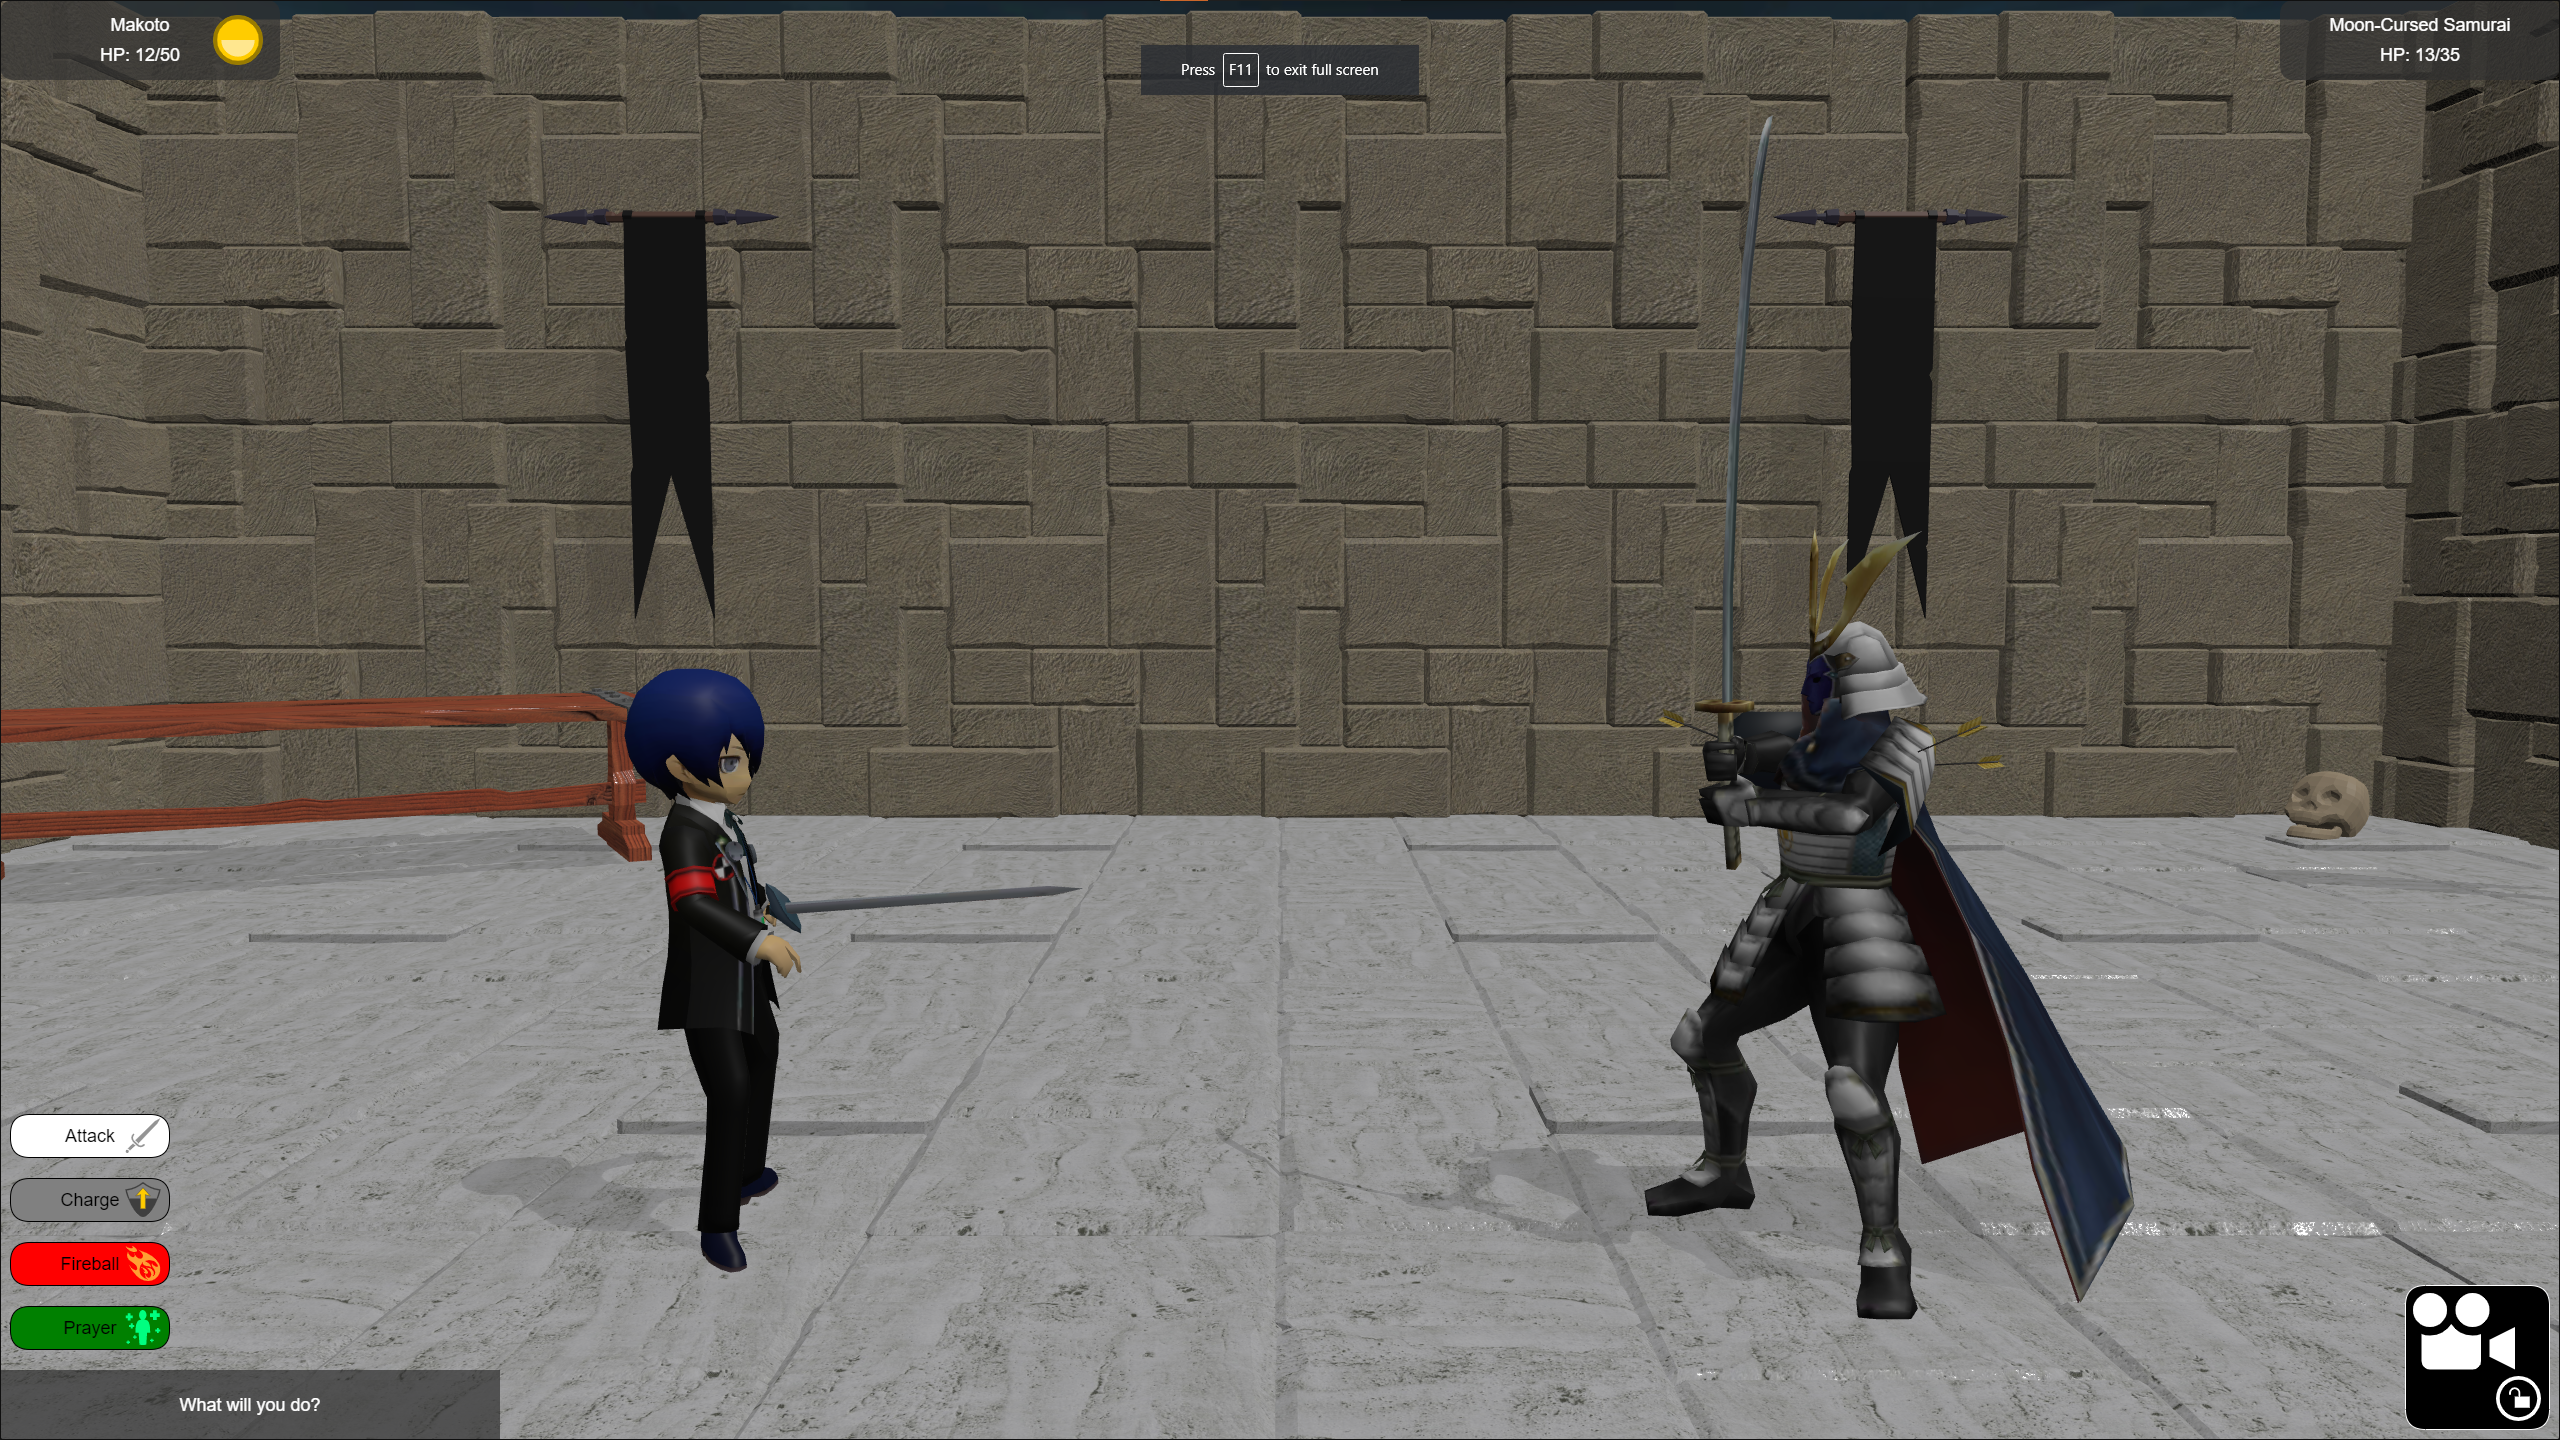
\includegraphics[width=0.9\textwidth]{images/ch4/battle-scene.png}
    }
    \caption{The battle scene}
\end{figure}

\section{Ending}

This scene is already fully discussed in the other chapters of this report and has no noteworthy technical details.

\begin{figure}[H]
    \centering
    \subfloat{
        \includegraphics[width=0.9\textwidth]{images/ch4/ending.png}
    }
    \caption{The ending scene}
\end{figure}

\section{Sky maps}
The sky maps are implemented using \texttt{BABYLON.PhotoDome} function, which creates a large sphere around the scene and attaches an equirectangular texture to its internal surface in order to create the illusion of a sky (or fog effect, if one wanted). There are two different images used in the game: the first one is used in most dungeon and battle scenes, while the second one is reserved for the boss.

\begin{figure}[H]
    \centering
    \subfloat{
        \includegraphics[width=0.9\textwidth]{images/ch4/skybox-dungeon.png}
    }
    \caption{The main sky map used in the dungeon and battle scenes}
\end{figure}

\begin{figure}[H]
    \centering
    \subfloat{
        \includegraphics[width=0.9\textwidth]{images/ch4/skybox-boss.png}
    }
    \caption{The boss sky map}
\end{figure}

\section{Camera and movement}

\subsection{Dungeon}

The camera used in the dungeon is a \texttt{Babylon.UniversalCamera}, which is a Babylon element we used to create a first-person perspective.
This camera is moved by the player using keyboard inputs, in two different ways: either using \textit{WASD} or the arrow buttons (see \autoref{sub:exploration-controls}).
The mouse is used to rotate the camera by clicking and dragging.
A gravity force has been applied to the camera, to forbid the player from flying.
The use of the function \texttt{engine.getDeltaTime()} when defining that character walking and running speed assures that all players experience the game moving at the same speed, independently of their framerate.

\subsection{Battle}
The camera used in the dungeon is a \texttt{Babylon.ArcRotateCamera}. The main difference from the dungeon camera is that this can only be rotated around a fixed point located in the center of the scene.
For this reason the keyboard here has no function, and only the mouse is used for rotating.
The camera's latitudinal movement is limited so that it doesn't go underground.
The UI also gives the player the possibility to lock the camera in its initial orientation.

\section{Collisions}
Most elements in the dungeon represent solid objects, so the player should be able to collide with them. However, because most meshes have a complex shape, we found it simpler and more reliable to assign invisible \textit{collision boxes} to those objects. They are simple invisible cuboids created with Babylon's \texttt{Box} primitive with dimensions similar to those of the associated object; they are then \textit{parented} to that object in order to inherit any displacement, rotation and scaling.

By creating flat boxes around the complex objects, and checking collisions with the former rather than the latter, the movement of the player in contact with other objects is smoothed significantly. In particular, the player never trips over all the irregularly-placed bricks of the floor, nor do they get stuck in wall corners.

In order to collide with these boxes, the player camera needs to have a collider as well, to simulate the body of the player. We set up an ellipsoid shape for this purpose.

Our usage of collisions has one basic principle: to stop the player from going where they shouldn't. In the case of walls and floors, they prevent them from falling outside of the map; in other cases, e.g. the locked gates and the spikes in the green room, collision is used as a game mechanic to prevent the player from "sequence breaking" the game. Even the enemies create an invisible collidable box that takes up a whole block for the same reason.


%!TEX root = main.tex

\chapter{Animations}

All animations in the project are realized in the JavaScript code and implemented as \texttt{BABYLON\\.Animation} objects, which are part of Babylon's own set of features for animation. We also use a simple wrapper library to simplify the handling of such objects.

\section{Our animation.js library}

In order to simplify the handling of the animations in our code, we wrote a small wrapper class for the Babylon Animation object. We called our new wrapper class Animation as well.

The main purpose of our wrapper is to save the length of the Babylon Animation it contains. Our module then offers a number of functions that take our wrappers as inputs and executes the contained Babylon animations by automatically setting the animation range based on the stored length. In this way we did not have to update the animation range of all function calls that execute a certain animation whenever we wanted to change the length of that animation.


\section{Character animations}

In our project we prototyped the animations in Blender. We use the keyframes values, obtained by manually manipulating the meshes using Blender tools, as reference to implement each animation in the code. After that we fine-tuned again their values to better adapt them to the scene. In order to make Blender references closest to the Babylon system, we had to set up the former to use the same order of Euler angles as Babylon, which was observed to be ZXY.

Although we always worked with Euler angles in Blender, when defining the final animations in the code we made use of both quaternions and Euler angles. The angles are used for simplicity when only a single component of the rotation vector changes, as well as a few instances where interpolating the angles worked better, while for animations that involved more than one Euler angles we decided to animate quaternions in order to get a more natural trajectory and avoid gimbal lock. We used the \texttt{BABYLON.Quaternion.FromEulerVector} function to convert between Euler and quaternions.

To animate the different meshes we use both \texttt{TransformNode} and \texttt{Bone} objects. Specifically, changes in the configuration of a node are persistent, so we used them when we wanted the final state of the object to be persistent, while the configuration of a bone is immediately reset to that of the corresponding node as soon as the animation ends for any reason. Furthermore, sometimes it happened that using the bones during the animation, the character would return to his initial position for a fraction of a second, also in this case we have worked around the problem using the nodes.
Generally, for the attacks we usually used the bones, while for animations such as Idle or Win we chose the nodes.

In order to easily access the relevant nodes and bones of the complex models, we created a JS object for each mesh to serve as a dictionary of bones for that mesh: they have the names of the relevant bones as keys and the corresponding \texttt{Bone} objects as values. Those objects can then be used to animate their rotation angles or quaternion, or retrieve the corresponding \texttt{TransformNode} object and do the same.

To finish most of the animations, we have applied some \textit{easing functions}. These allow us to define the progress rate of the animation between its beginning and its end, allowing us to speed it up or slow it down in some of its points. Most of the easing functions that we applied are quadratic or sine. Other, more peculiar easings will be pointed out explicitly below.

In the following sections we will describe the animation of each character.

\textit{\textbf{Note:} When executing a special action for the first time in each battle, the application may lag because of some initialization of the objects and particles involved, which the Babylon engine only performs at the time these elements are first used. This may prevent the animation from being shown cleanly the first time, but subsequent uses of the same special move will function normally.}



\subsection{Makoto}

\begin{wrapfigure}[14]{r}{0.5\textwidth}
    \centering
    \subfloat{
        \includegraphics[width=0.5\textwidth]{images/ch5/fireball.png}
    }
    \caption{Makoto casts Fireball}
    \label{fig:fireball}
\end{wrapfigure}

Makoto presents nine animations, four of them regards the actions that the user can takes on the battle (attack, fireball, charge, prayer), four more regard the passive movements in the battlefield (idle, flinch, death and victory) while the last one is appreciable at the end of game.



\begin{itemize}
    \item \textbf{Idle:} This animation is active when the character is not doing or undergoing any particular action and as long as this is true, the animation is repeated in loop. For Makoto, Idle consists of flexing his legs slightly, while his right leg moves forward and his left leg slightly backward.
    
    \item \textbf{Attack:} This is a simple animation, Makoto will swing his sword from the left to the right, twisting the torso in the meantime. This is a very quick animation, because it is meant to be used many times during the fight.
\end{itemize}

\begin{itemize}
    \item \textbf{Charge:} During this animation, Makoto stops moving his legs and moves its sword into a defensive position.

    \item \textbf{Fireball:}\footnote{This attack is referred to in the code with its work-in-progress codename, "Agi", which also has the benefit of being shorter and leaving the name "fireball" free for the sphere mesh to take.} This is a fairly long animation. The hero charges the magic by rotating the torso and right arm to the left, while the ambient light is lowered. When the shot is ready the character extends his arm towards the enemy and a fireball is thrown towards it (\autoref*{fig:fireball}). The fireball is a simple sphere, a Babylon primitive, with an emissive texture depicting the Sun on top. A light source moves along with in order to let the fireball light up the surrounding environment as well. When the fireball hits the enemy, it will explode. The explosion of fire is represented by the Particle System feature of Babylon, with a suitable fire-effect texture. During the animation the fireball's light will be the strongest active light source, making the animation really suggestive. At its end, the ambient light will return to normal.
    
    \item \textbf{Prayer:}\footnote{This attack is referred to in the code with its work-in-progress codename, "Dia", which also has the benefit of being shorter.} This, like Fireball, is a special animation, and to underline it also here we will see the ambient light decrease in intensity during its execution and return to normal at its end. To perform the animation Makoto will join hands, rotating his sword with the tip downwards (both for style reasons and to avoid penetration) and after that he will raise his head slightly upwards. At this point, particles will come out of the ground upwards, while healing light envelops Makoto and the ground below. Here, too, to simulate the effect of the cure, a bright green texture was applied over the particles.
    
    \item \textbf{Flinch:} This animation happens when the hero is hit by any attack and is not in a defensive position. It is quite short, both because it is designed to be reproduced often in battle, but also to simulate the quick reaction to the pain caused by the blow suffered. Makoto during Flinch will vibrate from the recoil, and will bend his torso and arms back towards his right shoulder. His head is also brought back slightly. However, the hero will quickly return to the starting position. The progression of the animation is driven by the easing function named \texttt{BackEase} with easing mode \texttt{EASEOUT}, with the result that Makoto will slightly overshoot the idle pose when returning from the flinching one, in order to show that regaining composure after being hit takes just a little more time.
    
    \item \textbf{Victory:} This animation is triggered whenever the player wins a battle. Makoto performs a final sword slash at nothing, and then puts his right hand in his pocket.
    
    \item \textbf{Death:} When Makoto loses a battle, he will first drop to his knees and then fall face down lifeless to the floor. It is a very simple animation, however, as in other animations, we refined it using the easing technique. In particular we used the \texttt{EASEIN} mode to give each part of the motion a slow, hesitant start (Makoto progressively losing his strength) and an abrupt stop (impact with the ground).
    
    \item \textbf{Ending animation:} At the end of the game, in front of his prize, we will see Makoto jump for joy on the spot. The character is translated upwards, reproducing a simple jump. The lower legs are bent back, the chin is raised slightly, the arms are raised to cheer, and to make the movement more natural, the back is bent slightly backward. All components are returned to the initial situation upon landing.

\end{itemize}



\subsection{Samurai}

This character has five animations: two attacks (normal attack, Luna special attack) and three other motions on the battlefield (idle, flinch, death).

\begin{itemize}
    \item \textbf{Idle:} A looping animation for when the Samurai is not undertaking any other action. Like Makoto, the animation consists in a little leg squatting, but to differentiate the two swordfighters, the Samurai holds his sword with two hands and in a different stance.
    
    \item \textbf{Attack:} A simple and quick animation in which the Samurai swings his katana to attack Makoto. It also twists its torso to make the hit a little more powerful.
    
    \item \textbf{Luna:} This attack has no displayed name, so it will be referred to by the name it was given in the code. The Samurai moves its sword precisely in front of it while the environmental light is dimmed to emphasize the upcoming lighting effects, and the sword and the decoration on top of the Samurai's helmet start glowing. Then the enemy raises his blade and quickly performs a downward slash, which causes an energy shockwave shaped like a crescent moon to be fired towards Makoto. When it hits, it triggers a particle effect representing the energy released by the hit and continues on its path, disappearing moments later. The projectile has an associated light source, allowing it to emit its own light and cast long shadows of the two combatants. At the end of the attack, the ambient lighting is restored.
    
    \item \textbf{Flinch:} A quick animation that triggers whenever the Samurai is hit by an attack. The enemy vibrates and recoils back, its secondary hand temporarily losing grip on the sword. Then, the warrior returns to its default position, with a little further recoil given by the \texttt{BackEase} transition function.
    
    \item \textbf{Death:} Triggers when the enemy loses all its HP. The Samurai falls to the ground in an elaborate but quick motion and dies unceremoniously.

\end{itemize}

\begin{figure}[H]
    \centering
    \subfloat{
        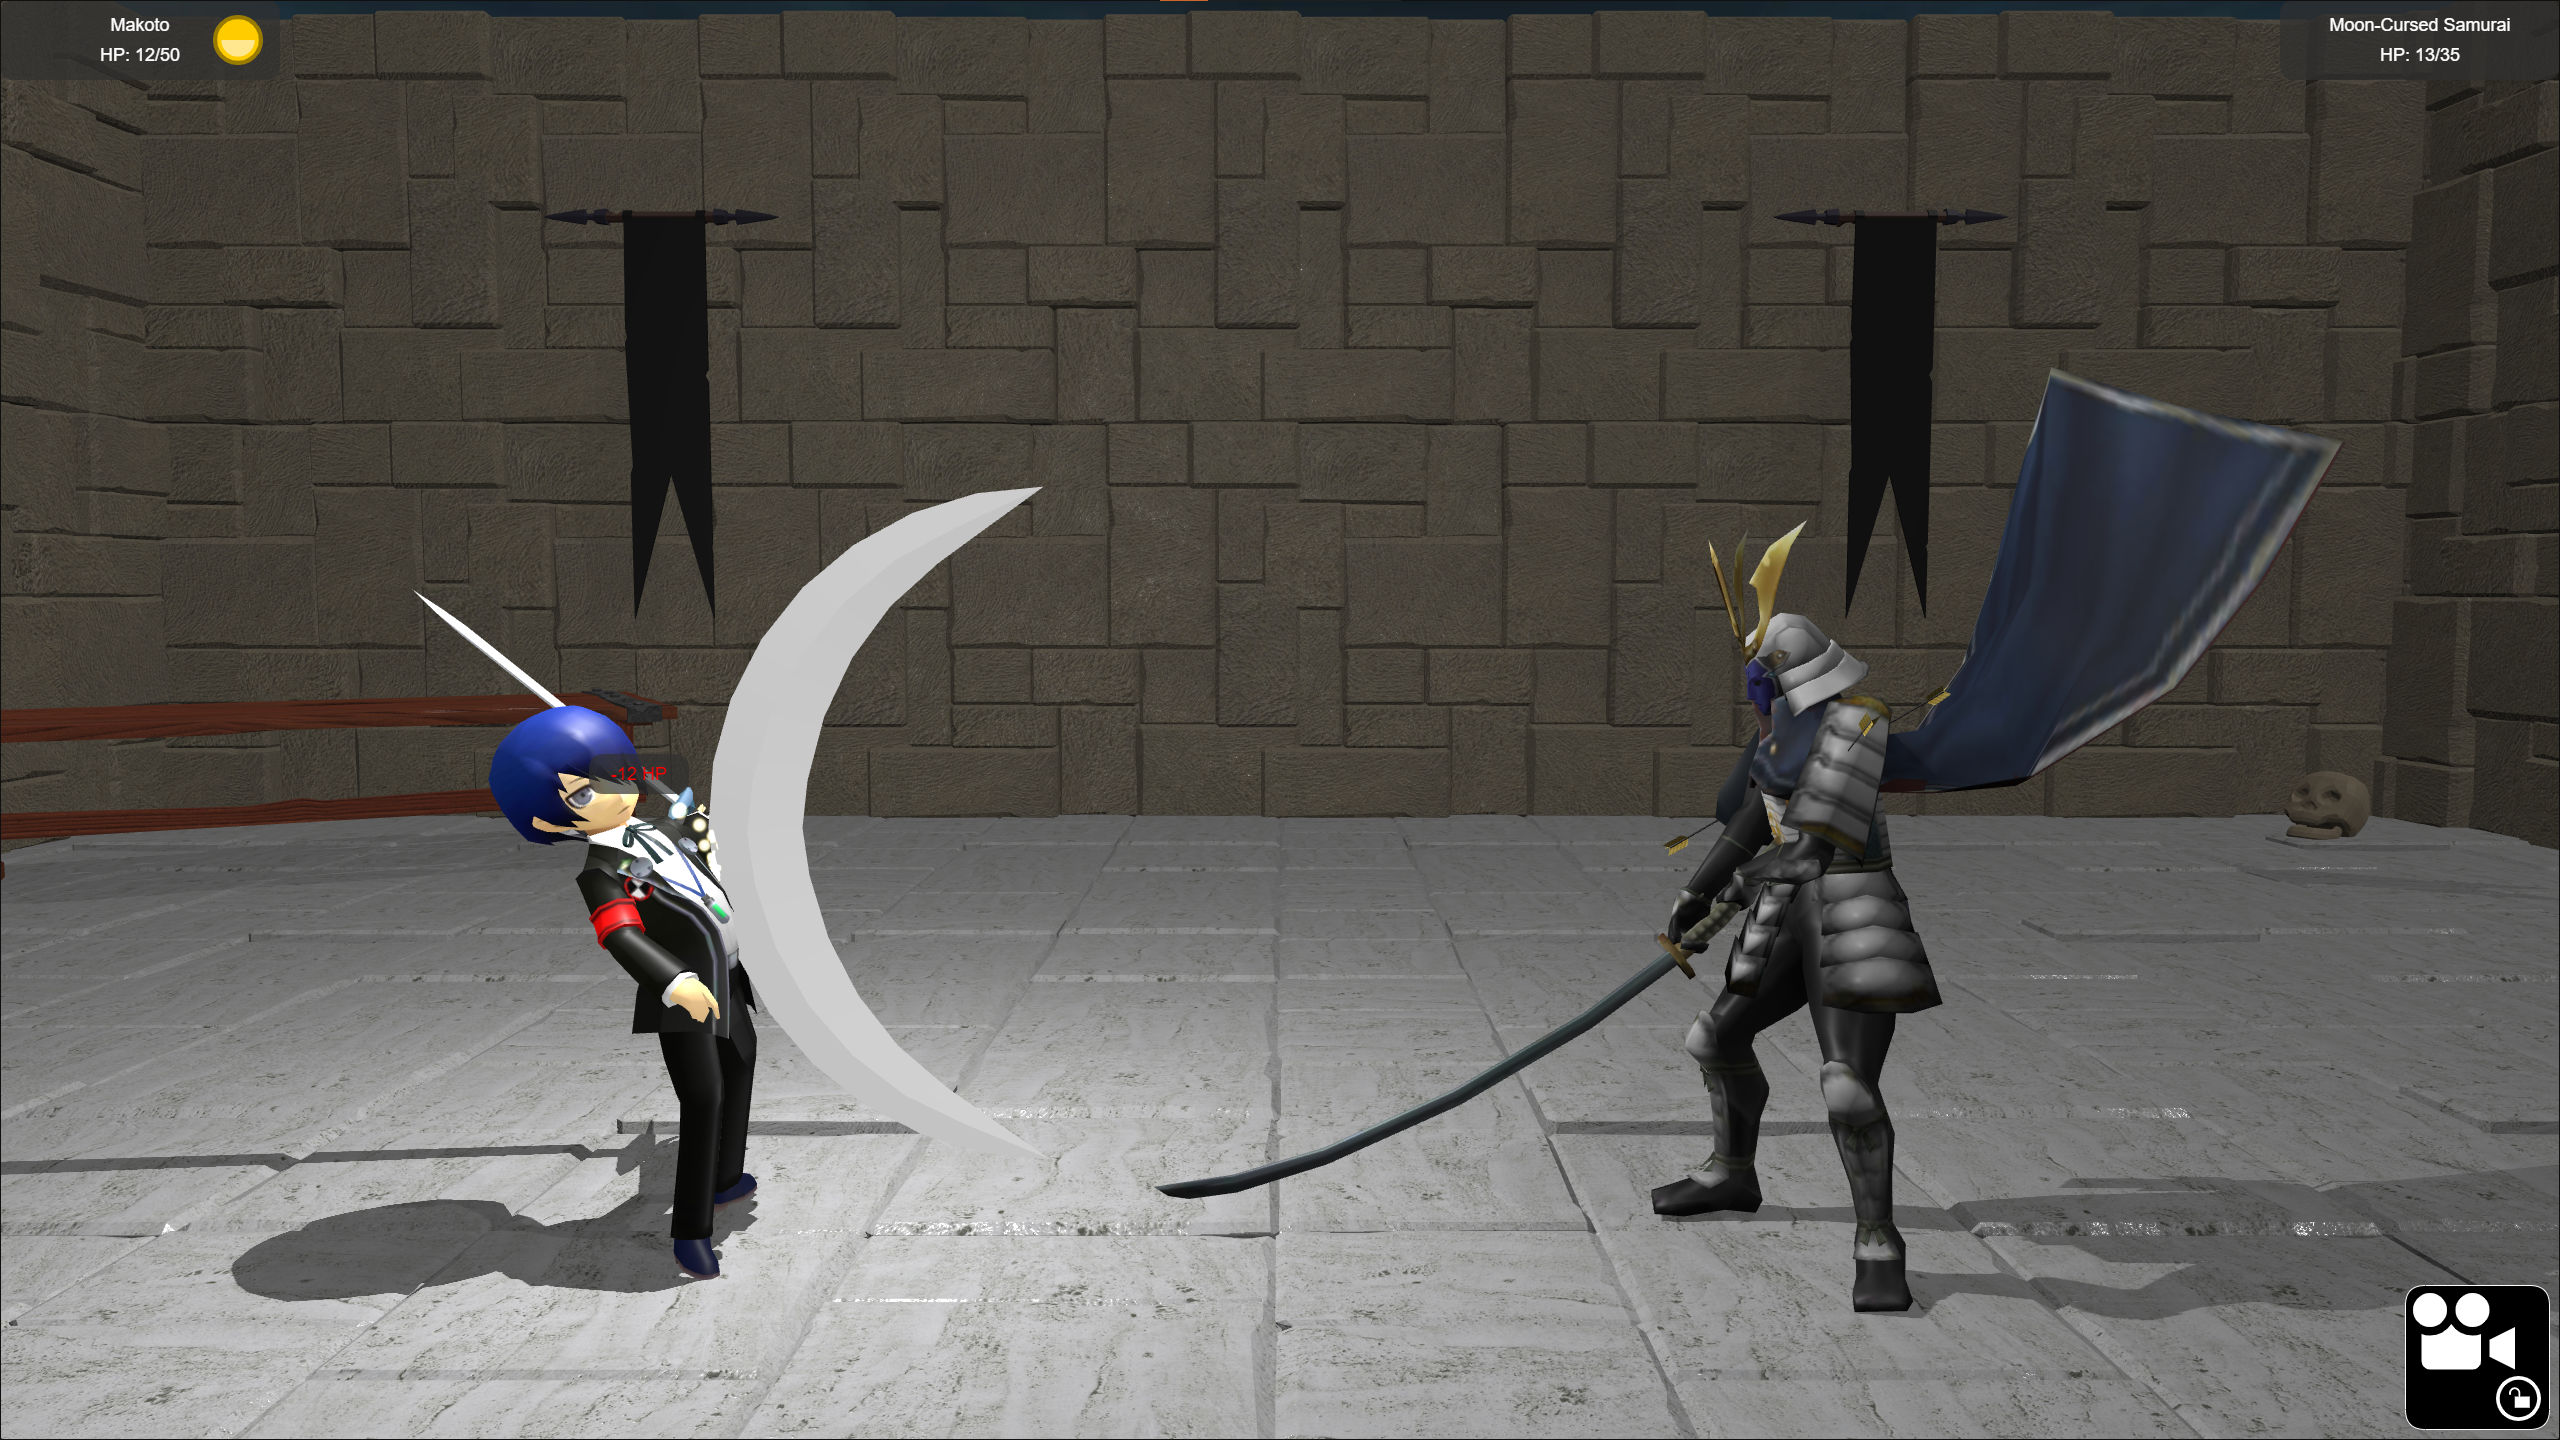
\includegraphics[width=0.7\textwidth]{images/ch5/luna.png}
    }
    \caption{Samurai attacks with Luna.}
    \label{fig:luna}
\end{figure}



\subsection{Boss}

\begin{wrapfigure}[19]{r}{0.5\textwidth}
    \centering
    \subfloat{
        \includegraphics[width=0.5\textwidth]{images/ch5/laser2.png}
    }
    \caption{The Boss attacks with its laser.}
    \label{fig:laser}
\end{wrapfigure}

This character has five animations: two attacks (normal attack, Laser special attack) and three other motions on the battlefield (idle, flinch, death).

\begin{itemize}
    \item \textbf{Idle:} A looping animation for when the Boss is not undertaking any other action. It simply consists of the monster's cape slightly expanding and shrinking in a breathing-like motion.
    
    \item \textbf{Attack:} A simple and quick animation for the normal attack. The demon raises the right side of its cape, then performs a sweeping motion with it and twists its equivalent of a spine to attack Makoto with the unnaturally sharp ends of the cape. The extremity of the cape also extends a little, in order to actually hit Makoto (rather than just performing the slashing motion and hit abstractly like the other characters do).
\end{itemize}

\begin{itemize}
    \item \textbf{Laser:} This attack has no displayed name, so it will be referred to by the name it was given in the code. After a few moments of concentration while the ambient light dims, the Boss opens its cape wide and bends forward in order to fire a laser beam from its mask. The laser pierces through Makoto, releases a particle effect, and emits light, casting the hero's shadow on the ground. At the end of the attack, the laser vanishes and the ambient lighting is restored.
    
    \item \textbf{Flinch:} The animation for when the enemy is hit by an attack. The Boss bends its equivalent of a spine backwards and sideways, while its cape opens as a result of this motion. Then the monster returns to its idle pose, with the usual recoil due to the \texttt{BackEase} effect.
    
    \item \textbf{Death:} Performed when the fiend is finally slain. An elaborate and dramatic animation: the Boss first recoils slightly in disbelief of its defeat, then it slowly starts to fall backwards as it stretches out its hand and its cape spreads wide; finally, after slowing down the motion for further dramatic effect near the end, the demon's body hits the ground, the stretched arm falls lifeless to its chest and the cape completes its fall.
\end{itemize}


\subsection{Closing note on character animations}

In order to allow each non-idle, non-flinch animation of a character to assume they will all start from the same initial pose without having the model abruptly snap to that starting pose with no transitions, those animations are only permitted to start between the end of an idle cycle and the beginning of the next one.

This means that between the moment the user clicks an action button (or the enemy starts its turn) and the moment the character performs their action there may be some waiting time depending on how close the current idle cycle is to ending, which is the cost we chose to pay in order to avoid the aforementioned rough transition. The wait can never exceed 1.6 seconds, the duration of one cycle.



\section{Other Animations}
In the \textit{dungeon} we have implemented some animations to make the game experience more dynamic and enjoyable. We have focused our attention on the principal objects present in the rooms.

\subsection{Keys and Padlock}

The animation of the keys is the first we encounter during the game. In its initial state, a key performs a simple floating animation like many other collectible objects in similar games do.

When the user interacts with the key by approaching and clicking it, the key will perform a simple transition animation to move in front of the camera and on the right side of the screen, as an object held by the player. The key remains in the same position and orientation relative to the camera as long as it is carried by the player: on the right side of the screen, very close to it to avoid penetration with the walls, and scaled down by a little to fit inside the screen.

Then, the user can use the key they are carrying on a padlock of the same color. When they do, a new animation is triggered, in which the key first flies to the lock, then turns to unlock the gate, then finally key, lock and gate bars all sink below the ground and disappear: the gate has been opened.

\begin{figure}[H]
      \centering
      \subfloat{
        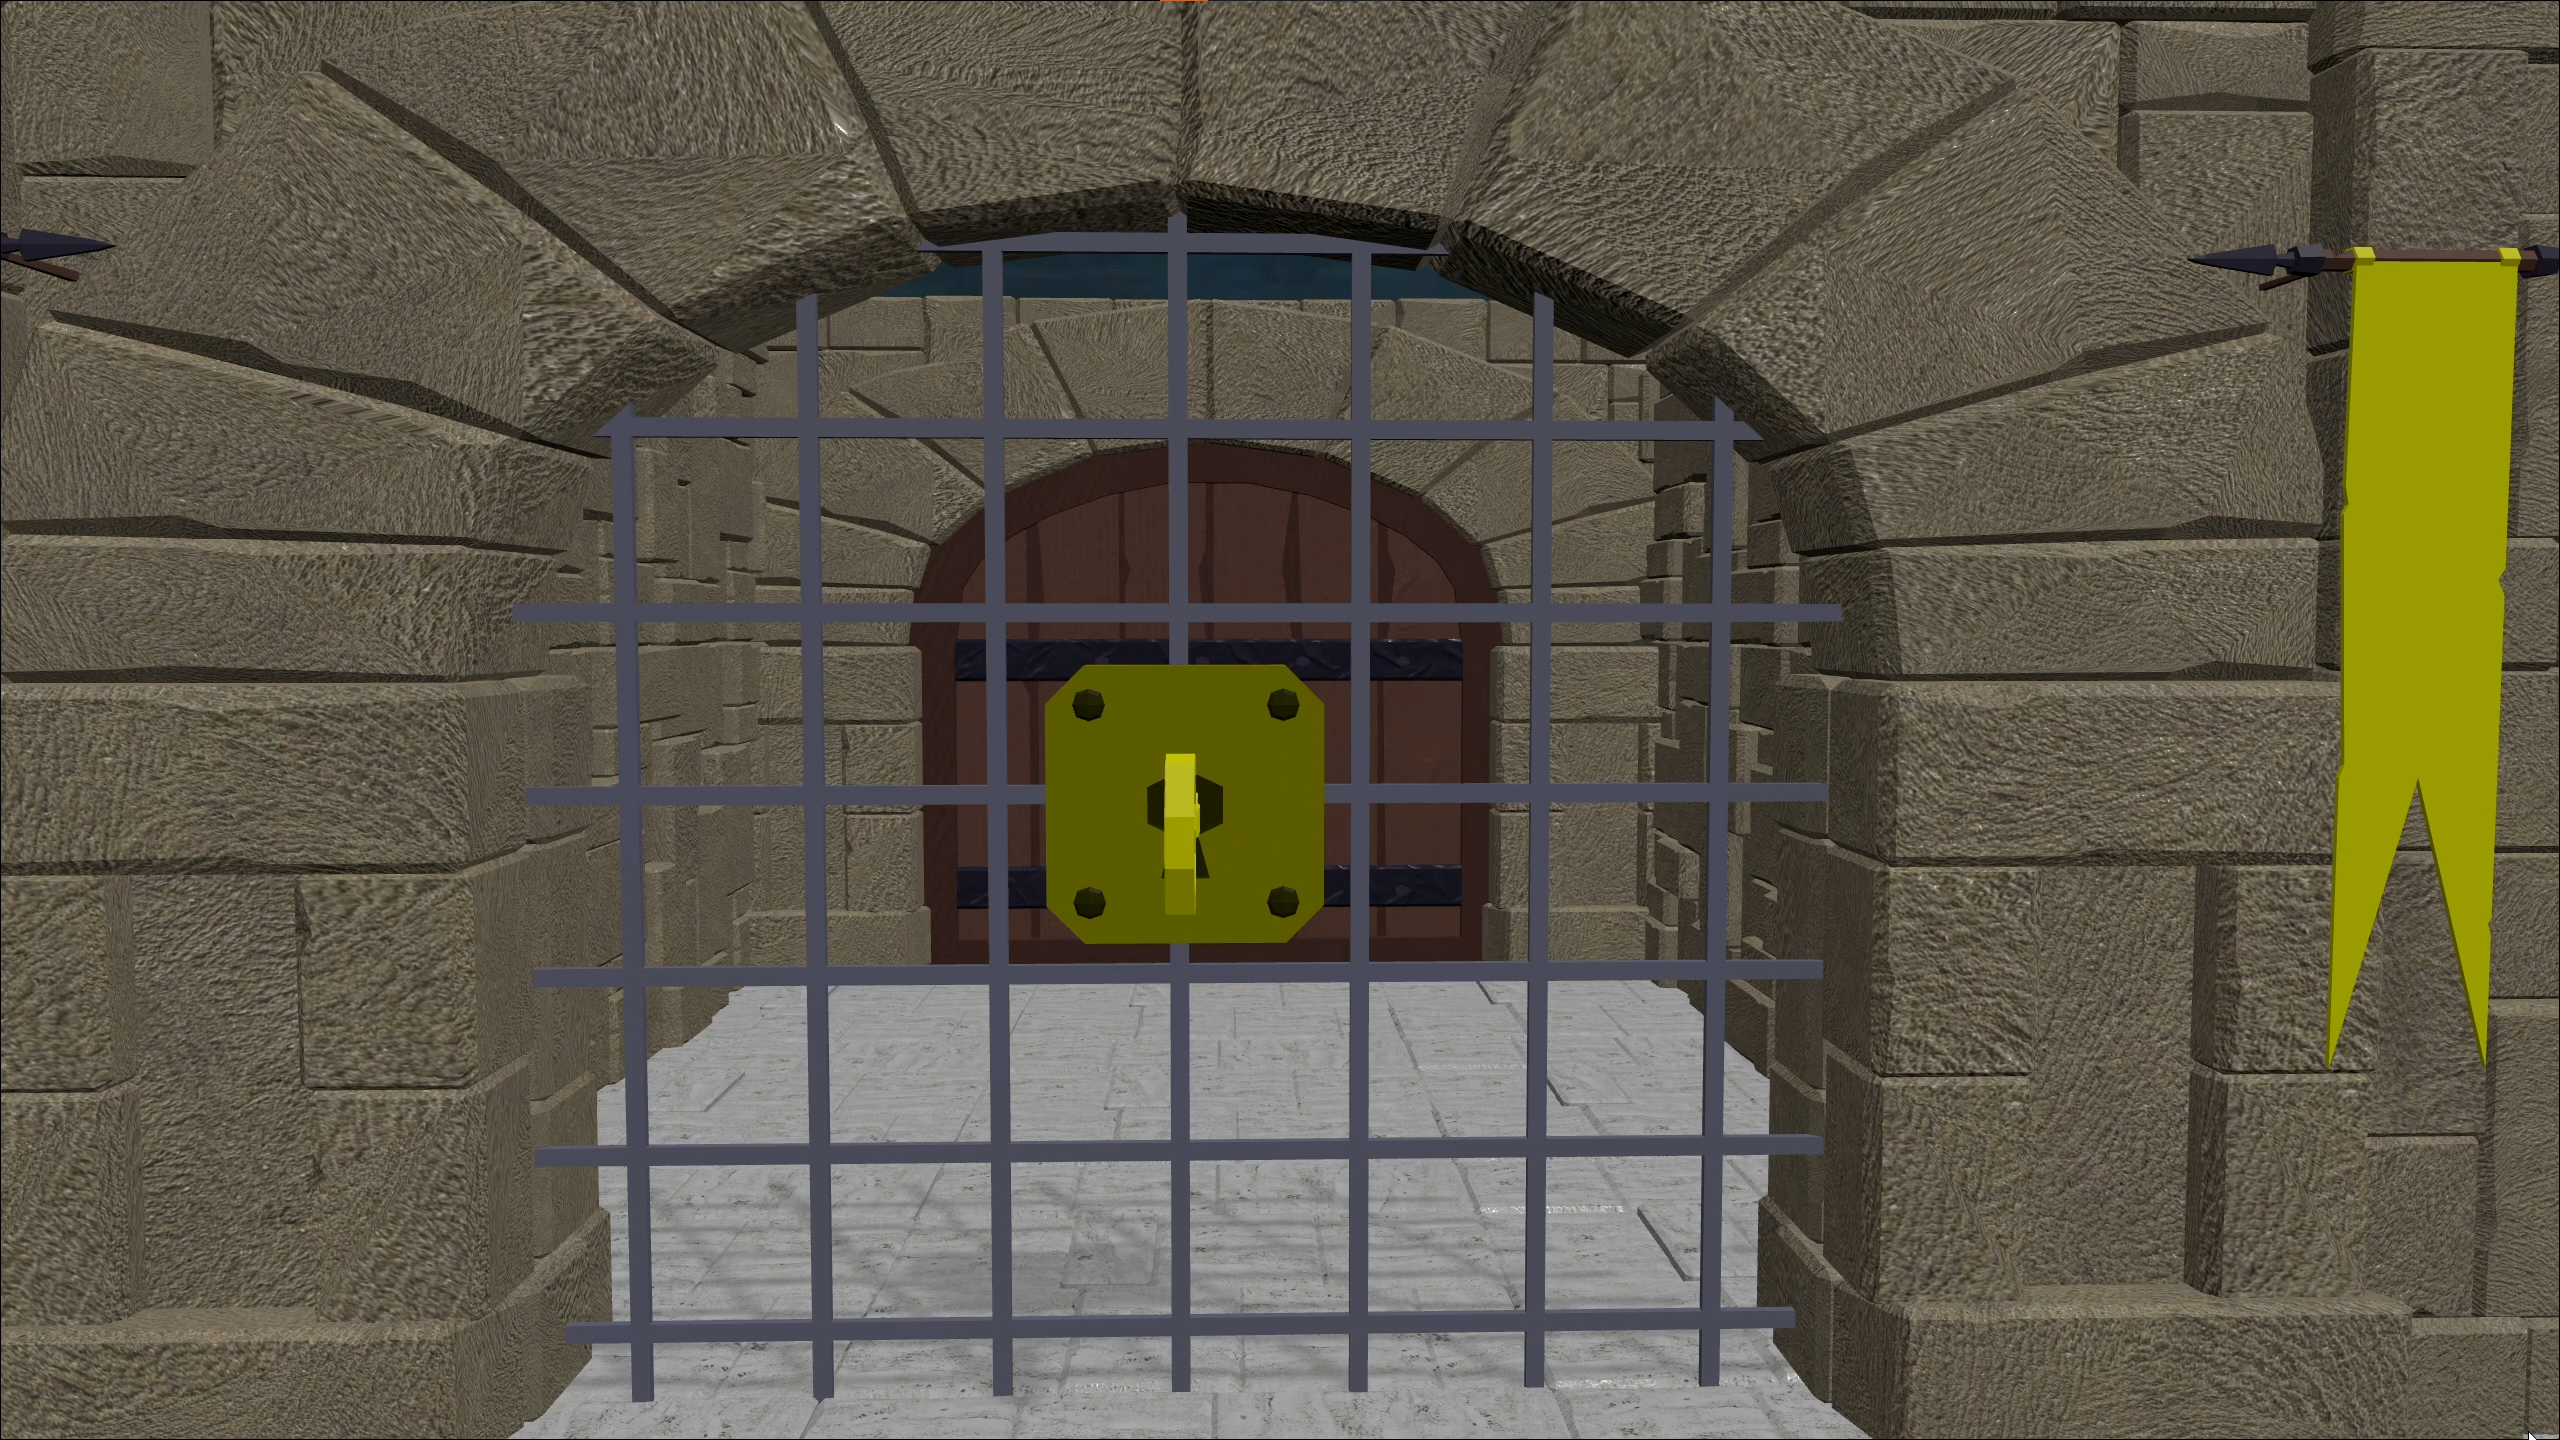
\includegraphics[width=0.4\textwidth]{images/ch5/key1.png}
    }
    \hspace{1cm}
    \subfloat{
        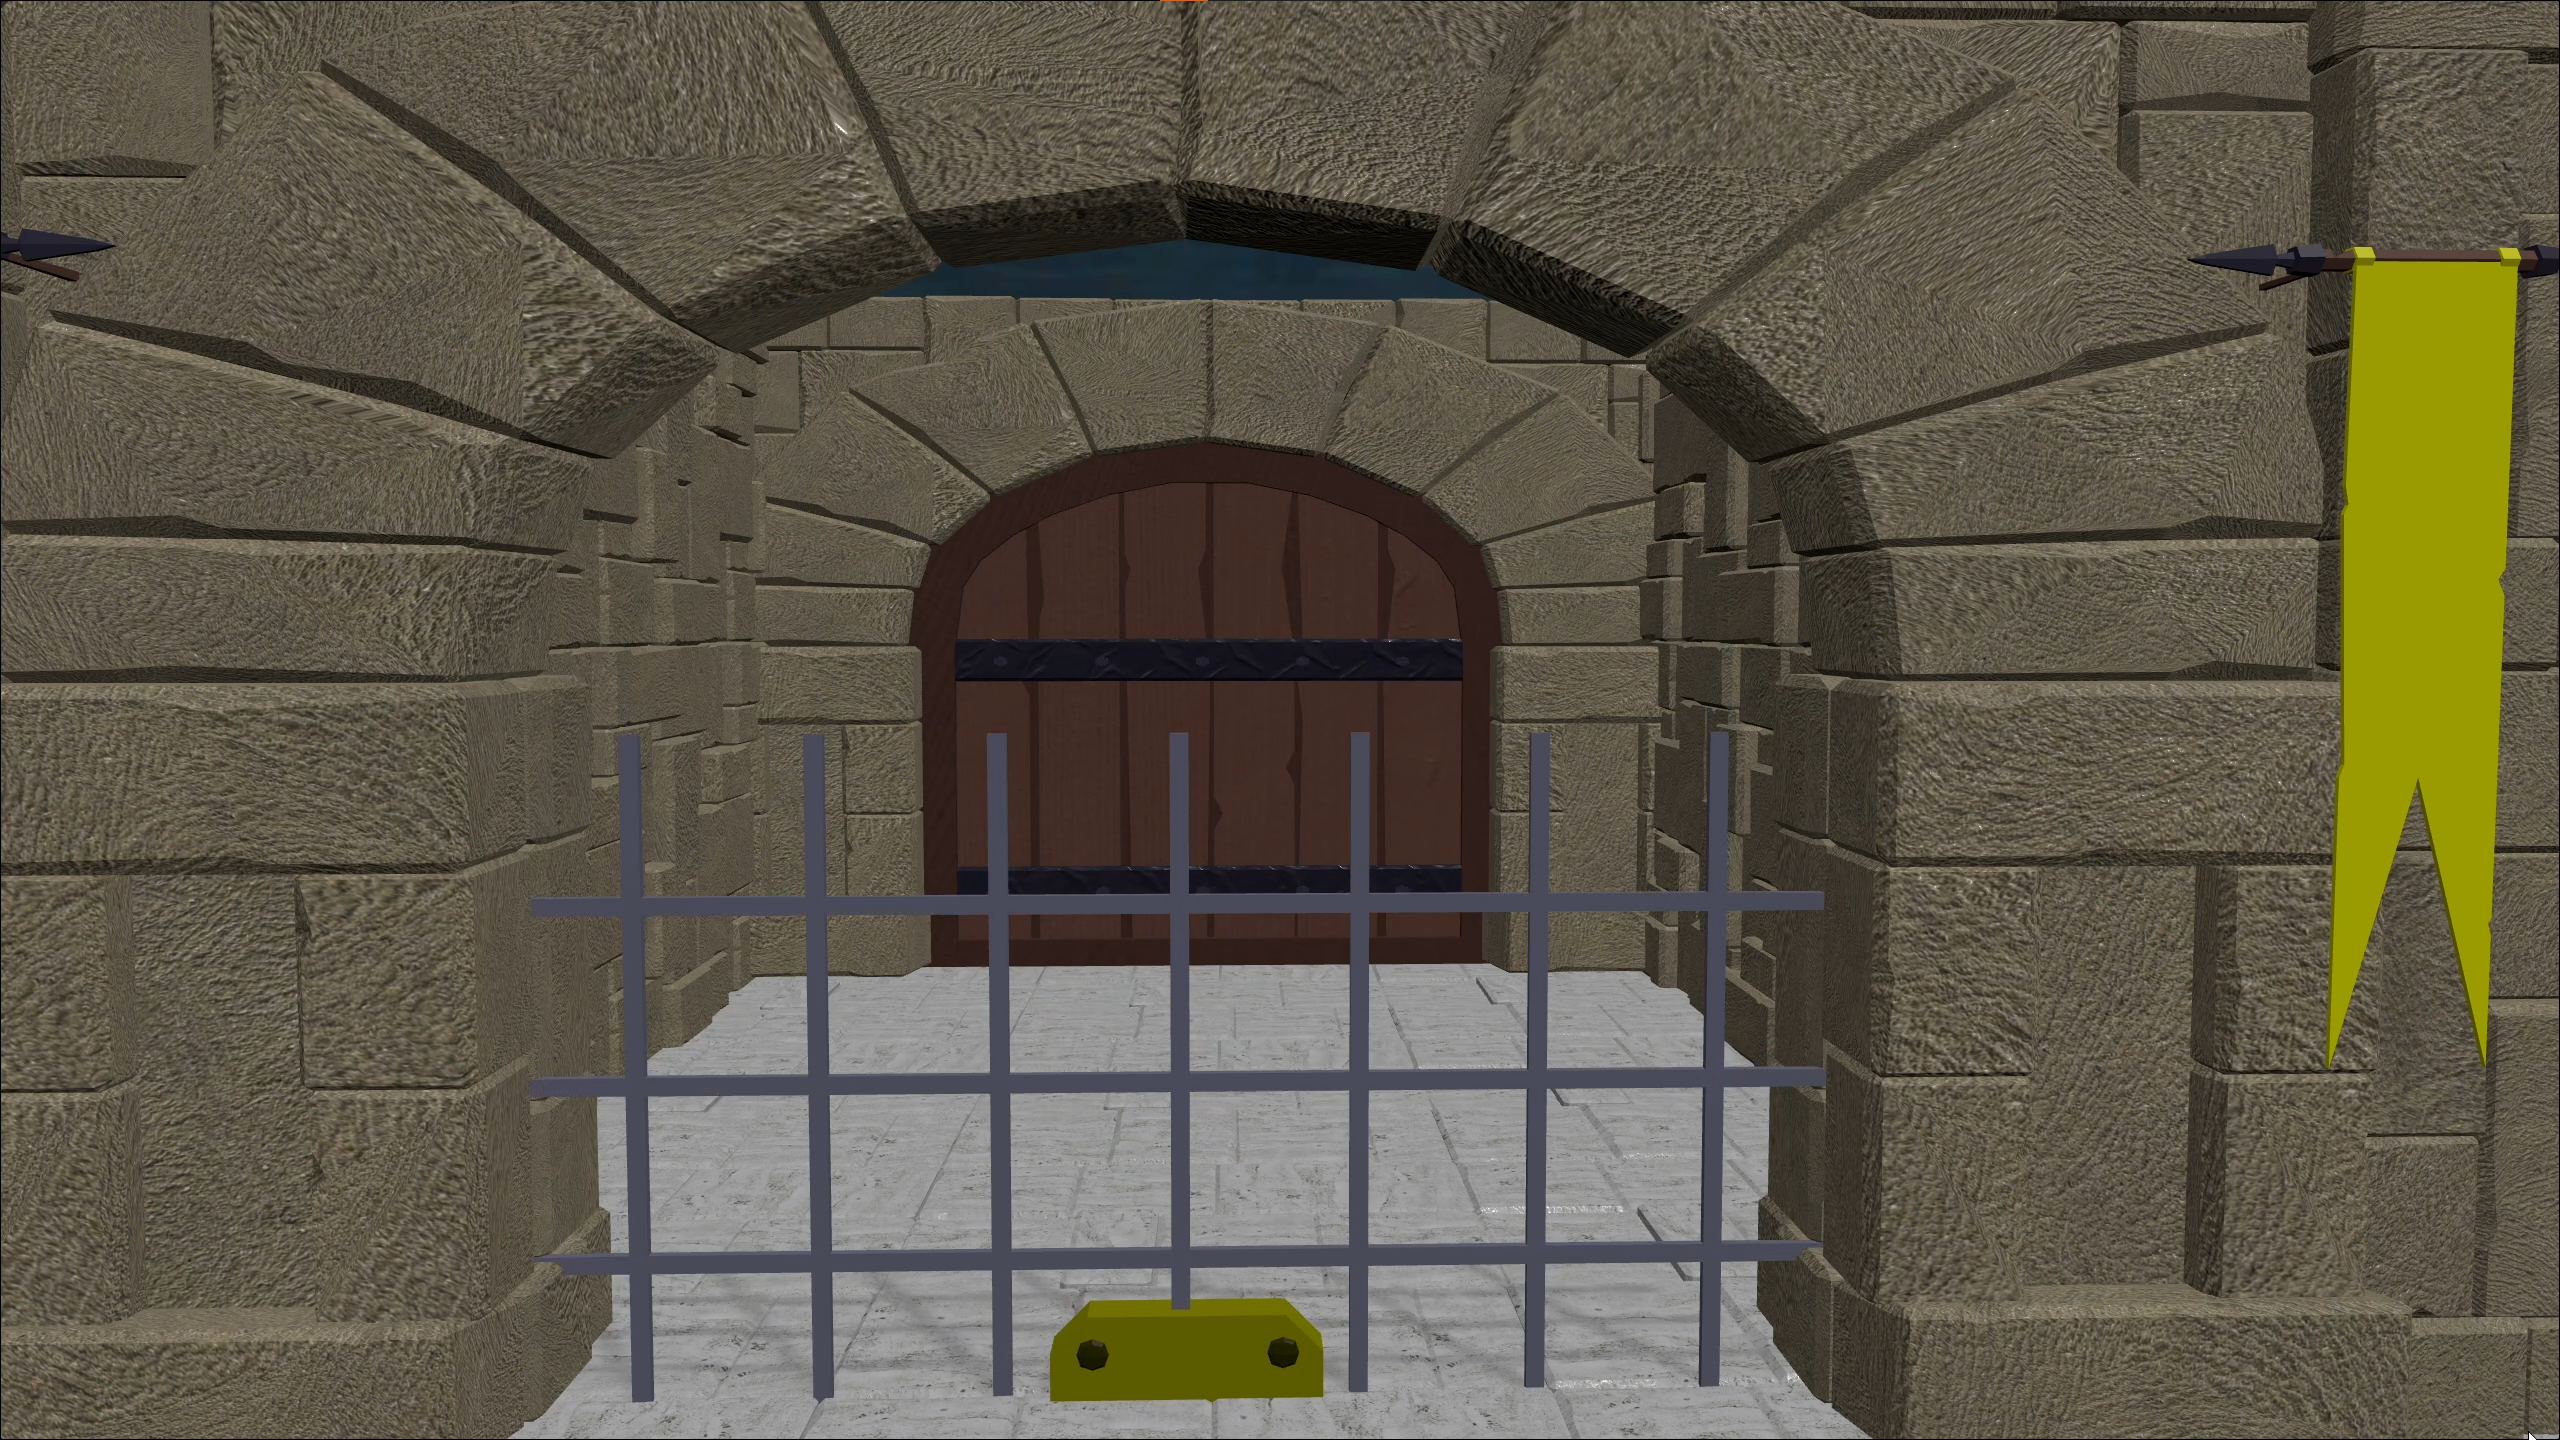
\includegraphics[width=0.4\textwidth]{images/ch5/key2.png}
    }
    \caption{Gate animation}
\end{figure}

\subsection{Door}

\begin{wrapfigure}[13]{r}{0.5\textwidth}
    \centering
    \subfloat{
        \includegraphics[width=0.5\textwidth]{images/ch5/door_open.jpg}
    }
    \caption{Door animation}
    \label{fig:door}
\end{wrapfigure}

Doors are the means by which the player moves between the different areas of the dungeon.

The animation of the door is very simple: when the user approaches and clicks it, the door swings open by rotating 90 degrees around its pivot. At the end of the animation, a scene change function is called to transport the user to the connected area.

Note, however, that in order to be able to approach certain doors the player will first have to unlock any intervening gates.


\subsection{Spike trap}


The purpose of this object is to serve as a surprise obstacle that activates when the user attempts to approach it, so that they are forced to take the detour route. It is \textit{not} intended to be a threat to the player's health. The spikes have two simple animations:

\begin{itemize}
    \item When the player comes closer than a set distance (presumably because they were trying to get to the key on the other side), the spikes will emerge from the ground in a very fast animation that uses a quintic easing function in order to be even faster.
    \item When the player takes the blue key, the trap is deactivated permanently, so the spikes sink back into the ground if they were up.
\end{itemize}

\begin{figure}[H]
    \centering
    \subfloat{
        \includegraphics[width=0.45\textwidth]{images/ch5/trap1.jpg} \hspace{5pt}
        \includegraphics[width=0.45\textwidth]{images/ch5/trap2.jpg}
    }
    \caption{spike trap before and after}
    \label{fig:trap1}
    \label{fig:trap2}
\end{figure}





%!TEX root = main.tex

\chapter{Lighting and Shadows}

\textit{Masks of Babylon} uses two broad types of lighting: environmental lighting, which is always present in dungeons and battles, and the lights emitted by the special attacks, which we use to create visual effects to accompany those actions.

\section{Environmental lighting}

The general lighting of the scenes is given by two basic light sources:

\begin{itemize}
    \item An \texttt{HemisphericLight} serves as a true ambient light and makes sure that every corner and object in the dungeon is decently lit for the user's benefit;
    \item A \texttt{DirectionalLight} is added in order to cast shadows, since the other one, as an ambient light, cannot.
\end{itemize}

The default intensity of these lights is slightly less that full power in order to be as coherent with the dark sky map as possible without making the environment too dark for the user. The intensity of the two lights is kept in sync at all times, so that we can animate them both by actively controlling only one.

Furthermore, the direction of these lights is slightly oblique, because a purely vertical direction would result in a worse lighting for some objects (especially the pedestal in the ending) and in trivially short shadows.

\section{Special attack lighting}

The light effects of the special actions make use of the other types of light source available in BabylonJS:

\begin{itemize}
    \item \textit{Fireball} uses a \texttt{PointLight} to represent the light emitted by the eponymous projectile. That is further represented by the emissive texture of the fireball's material.
    \item \textit{Prayer} uses two light sources to represent its healing light: an \texttt{HemisphericLight} that is set to affect only Makoto to fully envelop him in it, and a \texttt{PointLight} to illuminate the surrounding floor.
    \item \textit{Luna} uses a \texttt{PointLight} and an emissive material like \textit{Fireball}, and it also uses an \texttt{HemisphericLight} set to affect only Makoto to light him better in the moment he is hit.
    \item \textit{Laser} uses a \texttt{SpotLight} to represent the light emitted by the laser beam. Like the other offensive special actions, it also uses an emissive material for the beam mesh itself.
\end{itemize}

From a technical point of view, only one light per type was created for this kind of lighting: so all special actions share the same point light, the same spotlight and the same hemispherical light,\footnote{To clarify, the \texttt{HemisphericLight} of the special attacks is NOT the same object as the environmental one.} in order to spare some resources. Since no more than one of these moves is active at any given time, each of them takes possession of the lights it needs and sets their parameters as it begins.

The lights of the special attacks are set up to cast the shadows of nearby objects, notably the two combatants. This, combined with the fact that the environmental light gets dimmed to almost nothing for the whole duration of each special action, allows these moves to produce suggestive and emphasized lighting effects which enhance the graphical impact of the project.\\
The light of \textit{Prayer} casts no shadows because its light is supposed to be emitted by Makoto himself and is too weak to reach other objects, but the action still dims the environmental light for emphasis, as above.

\section{Shadows}

For the three lights that create shadows (the environmental \texttt{DirectionalLight} and the \texttt{Point} \texttt{Light} and \texttt{SpotLight} for the special attacks), the shadow casting is implemented by creating a \texttt{ShadowGenerator} object for each of those lights. This object holds the shadow map for the corresponding light source, whose resolution can be decided with a parameter, and it also offers the possibility to use some smoothing filters to increase the quality of the shadows. The \texttt{ShadowGenerator} then registers which objects in the scene should produce a shadow because of the associated light via the \texttt{addShadowCaster} method; and finally each object that should display the shadows does so by setting its own \texttt{receiveShadows} property.

Directional and spot lights cast shadows via simple projections, while point lights have to use a cube map, which is more expensive with respect to performance but allows them to cast shadows in all directions.\\
Because the battle scenes have few objects that should produce a shadow and the special attack lights are only active for a few seconds, we observed that using point lights with shadows have little impact on performance, which is why we used them where we needed and offered the possibility to reduce the quality level of the shadows.

We set most non-floor, non-wall objects as shadow casters and all floors and walls as shadow receivers. We decided against having walls cast shadows in order to let the floor have a better lighting, although this results in the shadow of some wall-mounted objects "floating" on the floor.\\
As an exception, the pedestal in the ending is both a shadow caster and a shadow receiver because it strongly needs to both cast its own shadow and receive the Cube of Babylon's.

The quality of the shadows is affected by the resolution of the shadow map and the type of smoothing filter used, if any. Specifically, the "Shadows" options found in the main menu correspond to the following combinations:

\begin{itemize}
    \item \textbf{Low Quality:} resolution 1024 and no filter. This results in blocky but efficient shadows, ideal for weaker GPUs. We decided against using a filter because the low resolution made the blurred borders look no better than the blocky ones.

    The only exception to this decision is the ending scene, where the shadow casters are few and close to each other, therefore the shadows are less blocky even at low resolution. Furthermore, the pedestal in that scene is both a shadow caster and a receiver, so a self-shadowing phenomenon is present. This scene uses a \textit{blurred close exponential shadow map} filter, which is the best for handling self-shadows.
    
    \item \textbf{High quality:} resolution 4096 and a smoothing filter depending on the scene: dungeons use \textit{percentage closer filtering}, battles use a \textit{blurred close exponential shadow map} like the ending. This dual filtering choice was made because the two types of scene have different needs, and each looked best with a different type of filter.
\end{itemize}

%!TEX root = main.tex

{
\let\clearpage\relax

\chapter{Other notable features}
}

\section{SceneManager}
Because the dungeon is split up into several scenes in order to lighten the burden on the rendering engine, and the battles happen in separate scenes than the dungeon, it is important that we can switch scenes and unload the previous one easily and often.

To that end we developed a so-called \texttt{SceneManager}, a singleton object with the role of holding the active scene object, rendering that scene, and handling requests to switch scenes by loading the new one and unloading the old one.

In order to go to a new non-dungeon scene, the \texttt{SceneManager} requires as argument an object that contains an asynchronous function to load that scene. We call such an object "Scene Builder", and that is what is exported by each JS file that defines a scene. Then the \texttt{SceneManager} disposes the current scene and starts loading the new one.

Transitioning to dungeon scenes is a little more complex, as it requires not only the destination scene builder but also the specific position and orientation the camera should be placed in, since some rooms have multiple entrance points. Apart from the different argument requirement, the process of disposing and loading the scenes is the same as non-dungeon scenes.

In the interim between when the old scene is disposed and when the new scene is ready, no scene is active, so the manager is instructed to not attempt to render anything. Instead, it displays a simple loading screen decorated with the logo of the game, a spinner, and a simple text informing the player of the loading in progress.

Finally, the \texttt{SceneManager} also offers a method to reload the current battle scene, essentially restarting the corresponding fight. This feature is used directly in the game over screen, and is implemented simply by saving the scene builder of the current scene so that it can be used later to reload it from scratch.


\section{Game state}
The \textit{game state} has a fundamental role in this project, it allows to maintain all the information about the state of the game the player is involved in. Indeed, it allows to move between different parts of the dungeon or in the battle scene without losing any information about what has been done in precedence. This is possible because we are using a global singleton object, that stores a persistent state for information
that needs to be constantly updated after each relevant action.
The information saved in the \textit{game state} are: 
\vspace{-10pt}
\begin{itemize}
\item which enemies have been defeated and should not appear again;
\item which object is carried by the player, if any;
\item the dungeon scene the player was in, as well as its position and orientation within it, when a fight starts;
\item which keys have been taken from their original spot and should not respawn; and which keys have been already used to unlock a gate, meaning that gate will never appear again;
\item whether the spike trap has never been triggered, has been activated once, or has been disabled permanently;
\item whether the story introduction screen has already been displayed in this playthrough.
\end{itemize}



\section{Battle turns}
The flow of battle is regulated by an object called \texttt{TurnSystem}. 

During each turn, both characters involved in the battle has the ability to notify the \texttt{TurnSystem} when they have terminated their animation for the turn: the active character will usually be executing an attack, while the other will have to flinch when they take the hit.

The \texttt{TurnSystem} object keeps track of who finished their own animation, and advances the battle to the next turn as soon as both characters are done, then resets its state and prepares to listen for the following turn.

In case the user selects a non-damaging action, i.e. Charge or Prayer, the player character immediately sends a notification to the \texttt{TurnSystem} on behalf of the enemy, since it will execute no animations in response to such a move.



\section{Battle UI hit markers}
During battle, the information related to the HP is shown in a more efficient and intuitive way thanks to the animations developed for the user interface. In fact, after each action that has consequences on the protagonist's or the enemy's HP, there is an animation that starts from the affected character and shows in a coloured square the HP that have been lost or gained during the turn.

Likewise, when the player character executes the Charge action, a similar square will appear to notify the user that they have been charged up and to point their attention to the charge state icon.



%!TEX root = main.tex

\chapter*{Resource attribution}

The following is a list of the sources of all models, textures, and other assets downloaded from the web to use in this project.

\section*{3D models}

\href{https://www.models-resource.com/3ds/personaqshadowofthelabyrinth/model/14509/}{Makoto} (player character), \href{https://www.models-resource.com/3ds/personaqshadowofthelabyrinth/model/14582/}{Samurai} (common enemy), \href{https://www.models-resource.com/3ds/personaqshadowofthelabyrinth/model/14564/}{Phantom Master} (boss enemy): provided by the Video Games Resource community. We removed some unnecessary elements.

Projectile for the Samurai's special attack: designed in Blender by us.

Cube of Babylon: our 3D reproduction of the current logo of BabylonJS.

All other non-primitive 3D models: original Blender files by the user Quaternius on the OpenGameArt forum: \href{https://opengameart.org/content/lowpoly-modular-dungeon-pack}{Modular Dungeon}, \href{https://opengameart.org/content/low-poly-rpg-pack}{Items}. UV mappings and some very minor adaptations by us.

\section*{Other}

Textures for Makoto, Samurai, Phantom Master: color textures provided along with the models. Other textures realized by us via simple editing of the color ones in GIMP.

Fireball emissive texture: a map of the Sun shot by the NASA STEREO probes in 2012. We could not find an official NASA source, possibly because of the age of the image, but this article (in Italian) explains its origin: \url{https://www.rivistageomedia.it/201210287530/Archivio/studio-del-sole-3d-dalle-sonde-stereo-della-nasa}

\href{https://www.textures-resource.com/nintendo_switch/mariokart8deluxe/texture/14725/}{Sky maps}: provided by the Video Game Resource community.

All other textures: \href{http://www.texturise.club/}{texturise.club}, whether taken directly or by combination of two or more textures from there.

All particles: \href{https://doc.babylonjs.com/toolsAndResources/assetLibraries/availableTextures}{BabylonJS Texture Library}.

Icons in the battle UI: The \href{https://opengameart.org/content/ui-pack-space-extension}{Charge State icon} is by the user Kenney on the OpenGameArt forum. The rest are from \href{https://game-icons.net/}{game-icons.net} and \href{https://iconmonstr.com/}{iconmonstr.com}, colored and slightly edited by us in Inkscape.


\end{document}